\documentclass{beamer}
\usepackage[utf8]{inputenc} % allow utf-8 input
\usepackage[T1]{fontenc}    % use 8-bit T1 fonts
\usepackage{hyperref}       % hyperlinks
\usepackage{url}            % simple URL typesetting
\usepackage{booktabs}       % professional-quality tables
\usepackage{amsfonts}       % blackboard math symbols
\usepackage{nicefrac}       % compact symbols for 1/2, etc.
\usepackage{microtype}      % microtypography
\usepackage{amsmath}
\usepackage{mathtools}
\usepackage{tikz}
\usetikzlibrary{calc}
\usetikzlibrary{bayesnet}
\usetikzlibrary{arrows}
\usepackage{color}
\usepackage{array}
\usepackage{dsfont}
\usepackage{multirow, graphicx}
 \usepackage{float}
\newcolumntype{C}[1]{>{\centering\arraybackslash}p{#1}}
\newcolumntype{R}[1]{>{\raggedleft\arraybackslash}p{#1}}
\newcolumntype{L}[1]{>{\raggedright\arraybackslash}p{#1}}
\usepackage{caption}
\usepackage{subfig}
\usepackage{pifont}
\usepackage{xcolor}
\usepackage{algorithm,algorithmic}
% \floatname{algorithm}{Procedure}
\renewcommand{\algorithmicrequire}{\textbf{Input:}}
\renewcommand{\algorithmicensure}{\textbf{Output:}}
\newcommand{\cmark}{\textcolor{green!80!black}{\ding{51}}}
\newcommand{\xmark}{\textcolor{red}{\ding{55}}}
\DeclareMathOperator*{\argmin}{argmin}
\urlstyle{same}
\usepackage{listings}
\usepackage[export]{adjustbox}
% \usetheme{Boadilla}

\title{Introduction to Seq2Seq Modeling}
% \subtitle{Using Beamer}
\author{Bill Watson}
\institute{S\&P Global}
\date{November 22, 2019}

\newenvironment{nospaceflalign*}
 {\setlength{\abovedisplayskip}{0pt}\setlength{\belowdisplayskip}{0pt}%
  \csname flalign*\endcsname}
 {\csname endflalign*\endcsname\ignorespacesafterend}

\AtBeginSection[]{
  \begin{frame}
  \vfill
  \centering
  \begin{beamercolorbox}[sep=8pt,center,shadow=true,rounded=true]{title}
    \usebeamerfont{title}\insertsectionhead\par%
  \end{beamercolorbox}
  \vfill
  \end{frame}
}

\begin{document}

\begin{frame}
\titlepage
\end{frame}


\begin{frame}
\frametitle{What are Sequence to Sequence Models?}
\begin{itemize}
  \item
\end{itemize}
\end{frame}

\begin{frame}
\frametitle{Common Applications for Seq2Seq Models}
\begin{itemize}
  \item Machine Translation
  \item Speech Recognition
  \item Text Summarization
\end{itemize}
\end{frame}

%%%%%%%%%%%%%%%%%%%%%%%%%%%%%%%%%%%%%%%%%%%%%%%%%%%%%%%%%%%%%%%%%%%%%%%%%%%%%%%%
\section{Encoder-Decoder Architecture}

\begin{frame}
\frametitle{Overview: Encoders and Decoders}
\begin{itemize}
  \item We have 2 sub-networks: an \textbf{Encoder} and a \textbf{Decoder}
  \item Encoders
  \begin{itemize}
    \item Give the source sentence meaning
  \end{itemize}
  \item Decoders
  \begin{itemize}
    \item Given the source sentence, emit a variable-length sequence
  \end{itemize}
  \item We will discuss how to connect the two for joint training
\end{itemize}
\end{frame}

\begin{frame}
\frametitle{Overview: Encoders and Decoders}
\begin{itemize}
  \item Encapsulation allows for flexible design choices:
  \begin{itemize}
    \item Embeddings
    \begin{itemize}
      \item Pre-trained
      \item DIY
    \end{itemize}
    \item Recurrent Layer
    \begin{itemize}
      \item Type
      \item Depth
      \item Directionality
    \end{itemize}
  \end{itemize}
\end{itemize}
\end{frame}

\begin{frame}
\frametitle{What makes an Encoder?}

\end{frame}

\begin{frame}
\frametitle{What makes a Decoder?}

\end{frame}


%%%%%%%%%%%%%%%%%%%%%%%%%%%%%%%%%%%%%%%%%%%%%%%%%%%%%%%%%%%%%%%%%%%%%%%%%%%%%%%%
\section{Word Embeddings: Practical Considerations}

\begin{frame}
\frametitle{Recap: Word Embeddings}

\end{frame}


\begin{frame}
\frametitle{Recap: Pretrained Word Embeddings}
\begin{itemize}
  \item Co-occurence Matrix
  \item Pointwise Mutal Information
  \item SVD Co-occurence
  \item Ngram
  \item CBOW, Skip Gram
  \item GloVe
  \item Sentence Embeddings: ELMo
\end{itemize}

\end{frame}


\begin{frame}
\frametitle{DIY Embeddings}
\begin{itemize}
  \item We can always train our own!
\end{itemize}
\end{frame}

\begin{frame}
\frametitle{Special Tokens for Sequence Modeling}
\begin{itemize}
  \item PAD $\rightarrow$ Padding / Masking
  \item UNK $\rightarrow$ Unkown words
  \item SOS $\rightarrow$ Start of Sentence
  \item EOS $\rightarrow$ End of Sentence
\end{itemize}
\end{frame}

\begin{frame}
\frametitle{Mangaging the Vocab Size}
\begin{itemize}
  \item Languages are unevely distributed
  \item Many rare words, names $\rightarrow$ inflates the size of the vocabulary
  \item \textbf{Problem:}
  \begin{itemize}
    \item Large embedding matricies for source, target language
    \item Large output layers for prediction and softmax
  \end{itemize}
  \item Naive Solution: Limit the vocab size to most frequent
\end{itemize}
% graph of zipfs law
\end{frame}

\begin{frame}
\frametitle{Morphology, Compounding, and Transliteration}
\begin{itemize}
  \item Morphological Analysis
  \begin{equation*}
    tweet, tweets, tweeted, tweeting, retweet, \hdots
  \end{equation*}
  \item Compund Splitting
  \begin{itemize}
    \item homework $\rightarrow$ home work
    \item website $\rightarrow$ web site
  \end{itemize}
  \item Names, Places, Proper Nouns
  \begin{itemize}
    \item Hoboken, Baltimore, Obama, Michelle
    \item Can do Transliteration
  \end{itemize}
\end{itemize}
\end{frame}

\begin{frame}
\frametitle{Handling Numbers}
\begin{itemize}
  \item Do we really need to encode every number? \textbf{NO!}
  \begin{equation*}
    \text{I pay 950.00 in May 2007} > \text{I pay 2007 in May 950.00}
  \end{equation*}
  \pause
  \item Solution 1: Replace with a NUM token, but
  \begin{equation*}
    \text{I pay NUM in May NUM} = \text{I pay NUM in May NUM}
  \end{equation*}
  \pause
  \item Solution 2: Replace each digit with a unique symbol, e.g. 5
  \begin{equation*}
    \text{I pay 555.55 in May 5555} > \text{I pay 5555 in May 555.55}
  \end{equation*}
  \item This reduces the need for embeddings, when we can simply do transliteration
\end{itemize}
\end{frame}

\begin{frame}
\frametitle{Factored Decomposition}

\end{frame}



\begin{frame}
\frametitle{Backoff}

\end{frame}



\begin{frame}
\frametitle{Character Models}

\end{frame}



\begin{frame}
\frametitle{BPE Subwords}

\end{frame}


%%%%%%%%%%%%%%%%%%%%%%%%%%%%%%%%%%%%%%%%%%%%%%%%%%%%%%%%%%%%%%%%%%%%%%%%%%%%%%%%
\section{Modeling Recurrent Relations}

\begin{frame}
\frametitle{Recap: Recurrent Layers}

\end{frame}

\begin{frame}
\frametitle{Vanilla RNNs}
\begin{equation*}
  h_t = \tanh \left( \overbrace{W_{ih} x_t + b_{ih}}^{input} + \underbrace{W_{hh} h_{t-1} + b_{hh}}_{hidden} \right)
\end{equation*}
\begin{itemize}
  \item $h_t$ is the hidden state at time $t$
  \item $x_t$ is the input at time $t$
  \item $h_{t-1}$ is the previous hidden state
  \item $h_0$ is initialized to $0$

\end{itemize}
\end{frame}

\begin{frame}
\frametitle{Long Short Term Memory (LSTM)}
\begin{equation*}
  \begin{split}
  \text{Gates} \rightarrow & \begin{cases}
  \begin{array}{ll}
              i_t = \sigma(W_{ii} x_t + b_{ii} + W_{hi} h_{t-1} + b_{hi}) \\
              f_t = \sigma(W_{if} x_t + b_{if} + W_{hf} h_{t-1} + b_{hf}) \\
              o_t = \sigma(W_{io} x_t + b_{io} + W_{ho} h_{t-1} + b_{ho}) \\
              g_t = \tanh(W_{ig} x_t + b_{ig} + W_{hg} h_{t-1} + b_{hg}) \\
  \end{array}
  \end{cases} \\
  \text{Outputs} \rightarrow & \begin{cases}
  \begin{array}{ll}
              c_t = f_t * c_{t-1} + i_t * g_t \\
              h_t = o_t * \tanh(c_t) \\
  \end{array}
\end{cases}
\end{split}
\end{equation*}

\begin{itemize}
  \item $h_t$ is the hidden state at time $t$
  \item $c_t$ is the cell state at time $t$
  \item $x_t$ is the input at time $t$

\end{itemize}
\end{frame}

\begin{frame}
\frametitle{Gated Recurrent Units (GRU)}
\begin{equation*}
  \begin{split}
  \text{Gates} \rightarrow & \begin{cases}
  \begin{array}{ll}
    r_t = \sigma(W_{ir} x_t + b_{ir} + W_{hr} h_{(t-1)} + b_{hr}) \\
    z_t = \sigma(W_{iz} x_t + b_{iz} + W_{hz} h_{(t-1)} + b_{hz}) \\
    n_t = \tanh(W_{in} x_t + b_{in} + r_t * (W_{hn} h_{(t-1)}+ b_{hn})) \\
  \end{array}
  \end{cases} \\
  \text{Outputs} \rightarrow & \begin{cases}
  \begin{array}{ll}
            h_t = (1 - z_t) * n_t + z_t * h_{(t-1)}
  \end{array}
\end{cases}
\end{split}
\end{equation*}
\begin{itemize}
  \item $h_t$ is the hidden state at time $t$
  \item $x_t$ is the input at time $t$
  \item $h_{t-1}$ is the previous hidden state
  \item $h_0$ is initialized to $0$
\end{itemize}

\end{frame}

\begin{frame}
\frametitle{Aside: Different Perspective on Deep Recurrent Models}
% insert koehn deep model nn-lm slide 37
\end{frame}



\begin{frame}
\frametitle{Aside: Dimensionality of Inputs and Outputs}

\begin{center}
\begin{tabular}{l|C{2.5cm}|C{2.5cm}|C{2.5cm}}
\toprule
\multicolumn{1}{c}{Type} &  \multicolumn{1}{c}{RNN} &  \multicolumn{1}{c}{LSTM} &  \multicolumn{1}{c}{GRU} \\
\midrule
In            & $B, L, H_{in}$              & $B, L, H_{in}$              & $B, L, H_{in}$ \\
\midrule
$h_{t-1}$ & $B, N_L \cdot N_D, H_{out}$ & $B, N_L \cdot N_D, H_{out}$ & $B, N_L \cdot N_D, H_{out}$ \\
$c_{t-1}$   & - & $B, N_L \cdot N_D, H_{out}$      & - \\
\midrule
$h_t$   & $B, N_L \cdot N_D, H_{out}$ & $B, N_L \cdot N_D, H_{out}$ & $B, N_L \cdot N_D, H_{out}$ \\
$c_t$     & - & $B, N_L \cdot N_D, H_{out}$ & - \\
\midrule
Out & $B, L, N_D \cdot H_{out}$   & $B, L, N_D \cdot H_{out}$   & $B, L, N_D \cdot H_{out}$ \\
\bottomrule
\end{tabular}
\end{center}

\begin{itemize}
  \item $B$ is the batch size
  \item $L$ is the sequence length
  \item $N_D$ is the number of directions
  \item $N_L$ is the number of layers
  \item $H_{in}, H_{out}$ are the input and hidden size
\end{itemize}
\end{frame}

\begin{frame}
\frametitle{Aside: The Influence of Padding in RNNs}

\end{frame}

\begin{frame}
\frametitle{Right to Left Sequence Modeling}
\begin{itemize}
  \item So far, we've only seen Left to Right Sequencing
  \item Why not Right to Left?
\end{itemize}
\end{frame}

\begin{frame}
\frametitle{Bidirectional Sequence Modeling}
\begin{itemize}
  \item Why not both directions?
  \item We concatenate the results of each direction together
\end{itemize}
\end{frame}

%%%%%%%%%%%%%%%%%%%%%%%%%%%%%%%%%%%%%%%%%%%%%%%%%%%%%%%%%%%%%%%%%%%%%%%%%%%%%%%%


\section{Putting together an Encoder}

\begin{frame}
\frametitle{The Components of an Encoder}
\begin{figure}[ht!]
  \centering
  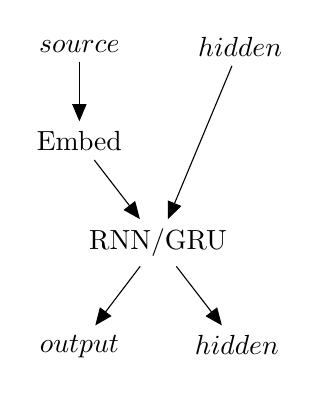
\begin{tikzpicture}

    % Define nodes
    \node[rectangle] (rnn) {RNN/GRU};
    \node[rectangle, below=0.75cm of rnn, xshift=-1cm] (out) {$output$};
    \node[rectangle, below=0.75cm of rnn, xshift=1cm] (hidden2) {$hidden$};
    \node[rectangle, above=0.75cm of rnn, xshift=-1cm] (embed) {Embed};
    \node[rectangle, above=0.75cm of embed] (input) {$source$};
    \node[rectangle, right=0.75cm of input] (hidden1) {$hidden$};

    % Connect the nodes
    \edge {input} {embed};
    \edge {embed, hidden1} {rnn};
    \edge {rnn} {out, hidden2};

  \end{tikzpicture}
  \caption{Model Architecture for Encoder.}
  \label{fig:encoder}
\end{figure}
\end{frame}


%%%%%%%%%%%%%%%%%%%%%%%%%%%%%%%%%%%%%%%%%%%%%%%%%%%%%%%%%%%%%%%%%%%%%%%%%%%%%%%%
\section{Putting together an Decoder}

\begin{frame}
\frametitle{The Components of a Decoder}
\begin{figure}[ht!]
  \centering
  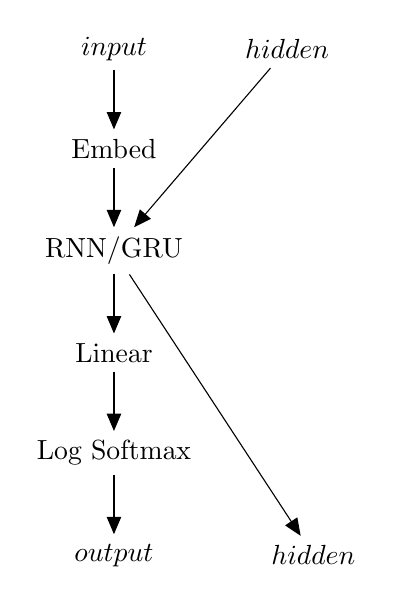
\begin{tikzpicture}

    % Define nodes
    \node[rectangle] (rnn) {RNN/GRU};
    \node[rectangle, above=0.75cm of rnn] (embed) {Embed};
    \node[rectangle, above=0.75 of embed] (input) {$input$};
    \node[rectangle, right=1cm of input] (hidden1) {$hidden$};
    \node[rectangle, below=0.75cm of rnn] (linear) {Linear};
    \node[rectangle, below=0.75cm of linear] (logs) {Log Softmax};
    \node[rectangle, below=0.75cm of logs] (out) {$output$};
    \node[rectangle, right=1.25cm of out] (hidden2) {$hidden$};

    % Connect the nodes
    \edge {input} {embed};
    \edge {embed, hidden1} {rnn};
    \edge {rnn} {linear, hidden2};
    \edge {linear} {logs};
    \edge {logs} {out};

  \end{tikzpicture}
  \caption{Decoder with No Attention.}
  \label{fig:decoder-no-attn}
\end{figure}
\end{frame}

\begin{frame}
\frametitle{Connecting the Encoder}
\begin{figure}[ht!]
  \centering
  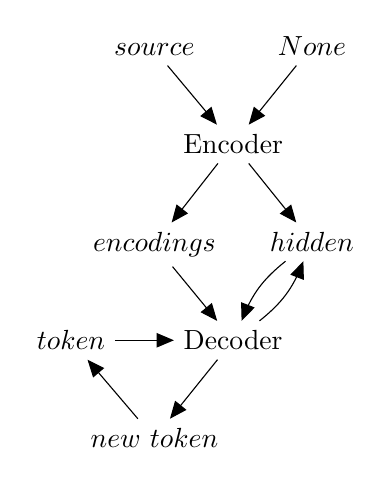
\begin{tikzpicture}

    % Define nodes
    \node[rectangle] (encoder) {Encoder};
    \node[rectangle, below=2cm of encoder] (decoder) {Decoder};
    \node[rectangle, above=0.75cm of encoder, xshift=-1cm] (s) {$source$};
    \node[rectangle, above=0.75cm of encoder, xshift=1cm] (hidden1) {$None$};
    \node[rectangle, below=0.75cm of encoder, xshift=-1cm] (out1) {$encodings$};
    \node[rectangle, below=0.75cm of encoder, xshift=1cm] (hidden2) {$hidden$};
    \node[rectangle, left=0.75cm of decoder] (t) {$token$};
    \node[rectangle, below=0.75cm of decoder, xshift=-1cm] (out2) {$new$ $token$};
    % \node[rectangle, below=0.75cm of decoder, xshift=1cm] (hidden3) {$hidden$};

    % Connect the nodes
    \edge {s, hidden1} {encoder};
    \edge {encoder} {out1, hidden2};
    \edge {out1, t} {decoder};
    \edge {decoder} {out2};
    \edge {out2} {t};
    \path [->] (decoder) edge [bend right=15] node {} (hidden2);
    \path [->] (hidden2) edge [bend right=15] node {} (decoder);

  \end{tikzpicture}
  \caption{Model Architecture Overview for Encoder-Decoder.}
  \label{fig:encoder-decoder}
\end{figure}
\end{frame}

\begin{frame}
\frametitle{Decoder Inference: Making Predictions}

\end{frame}

\begin{frame}
\frametitle{Teacher Forcing}

\end{frame}


%%%%%%%%%%%%%%%%%%%%%%%%%%%%%%%%%%%%%%%%%%%%%%%%%%%%%%%%%%%%%%%%%%%%%%%%%%%%%%%%
\section{Training Considerations}

\begin{frame}
\frametitle{Increasing Throughput through Batching}
\begin{figure}
  \centering
  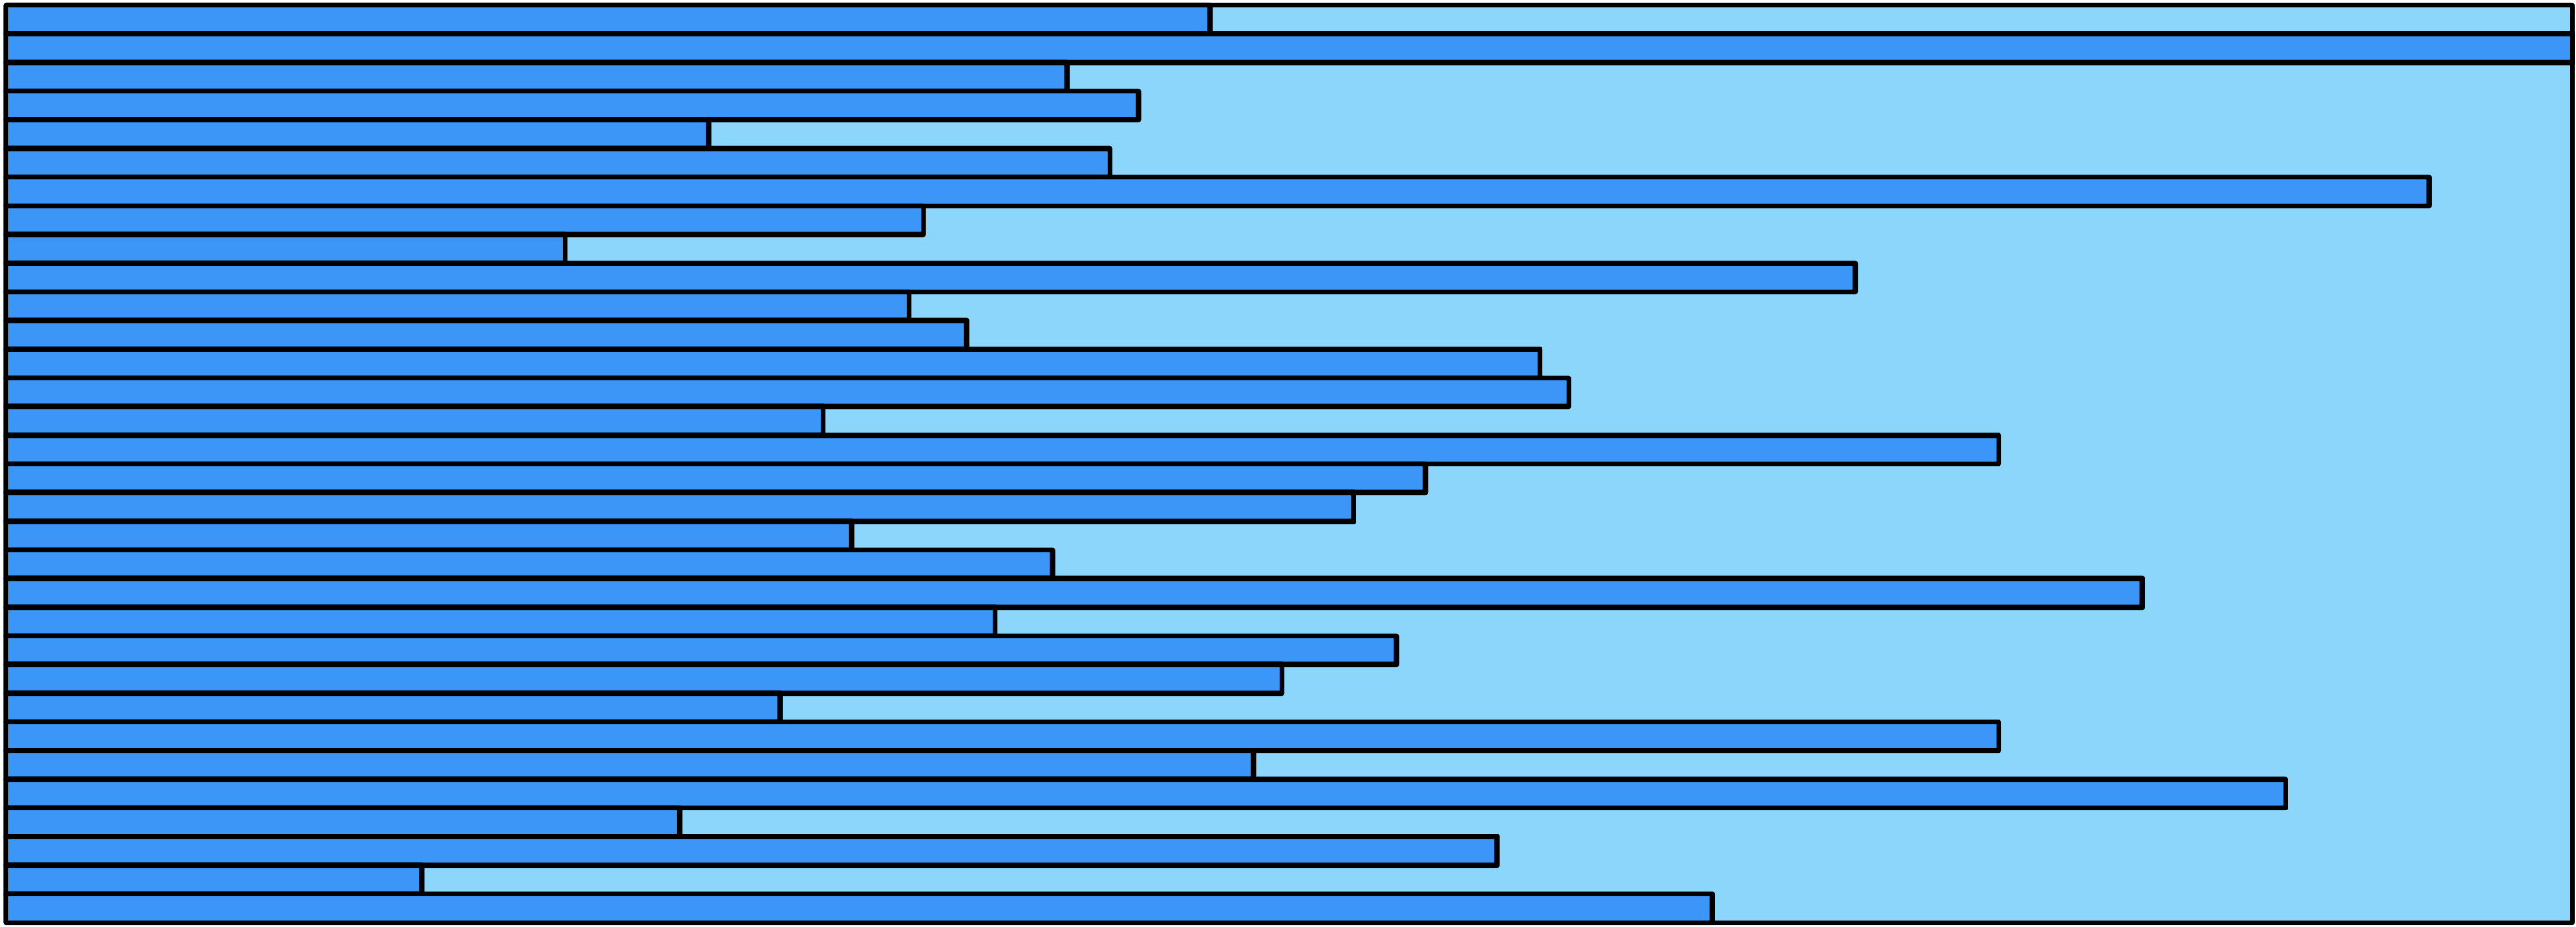
\includegraphics[width=4.5cm, valign=c]{assets/full_batch}
  \quad
  $\Longrightarrow$
  \quad
  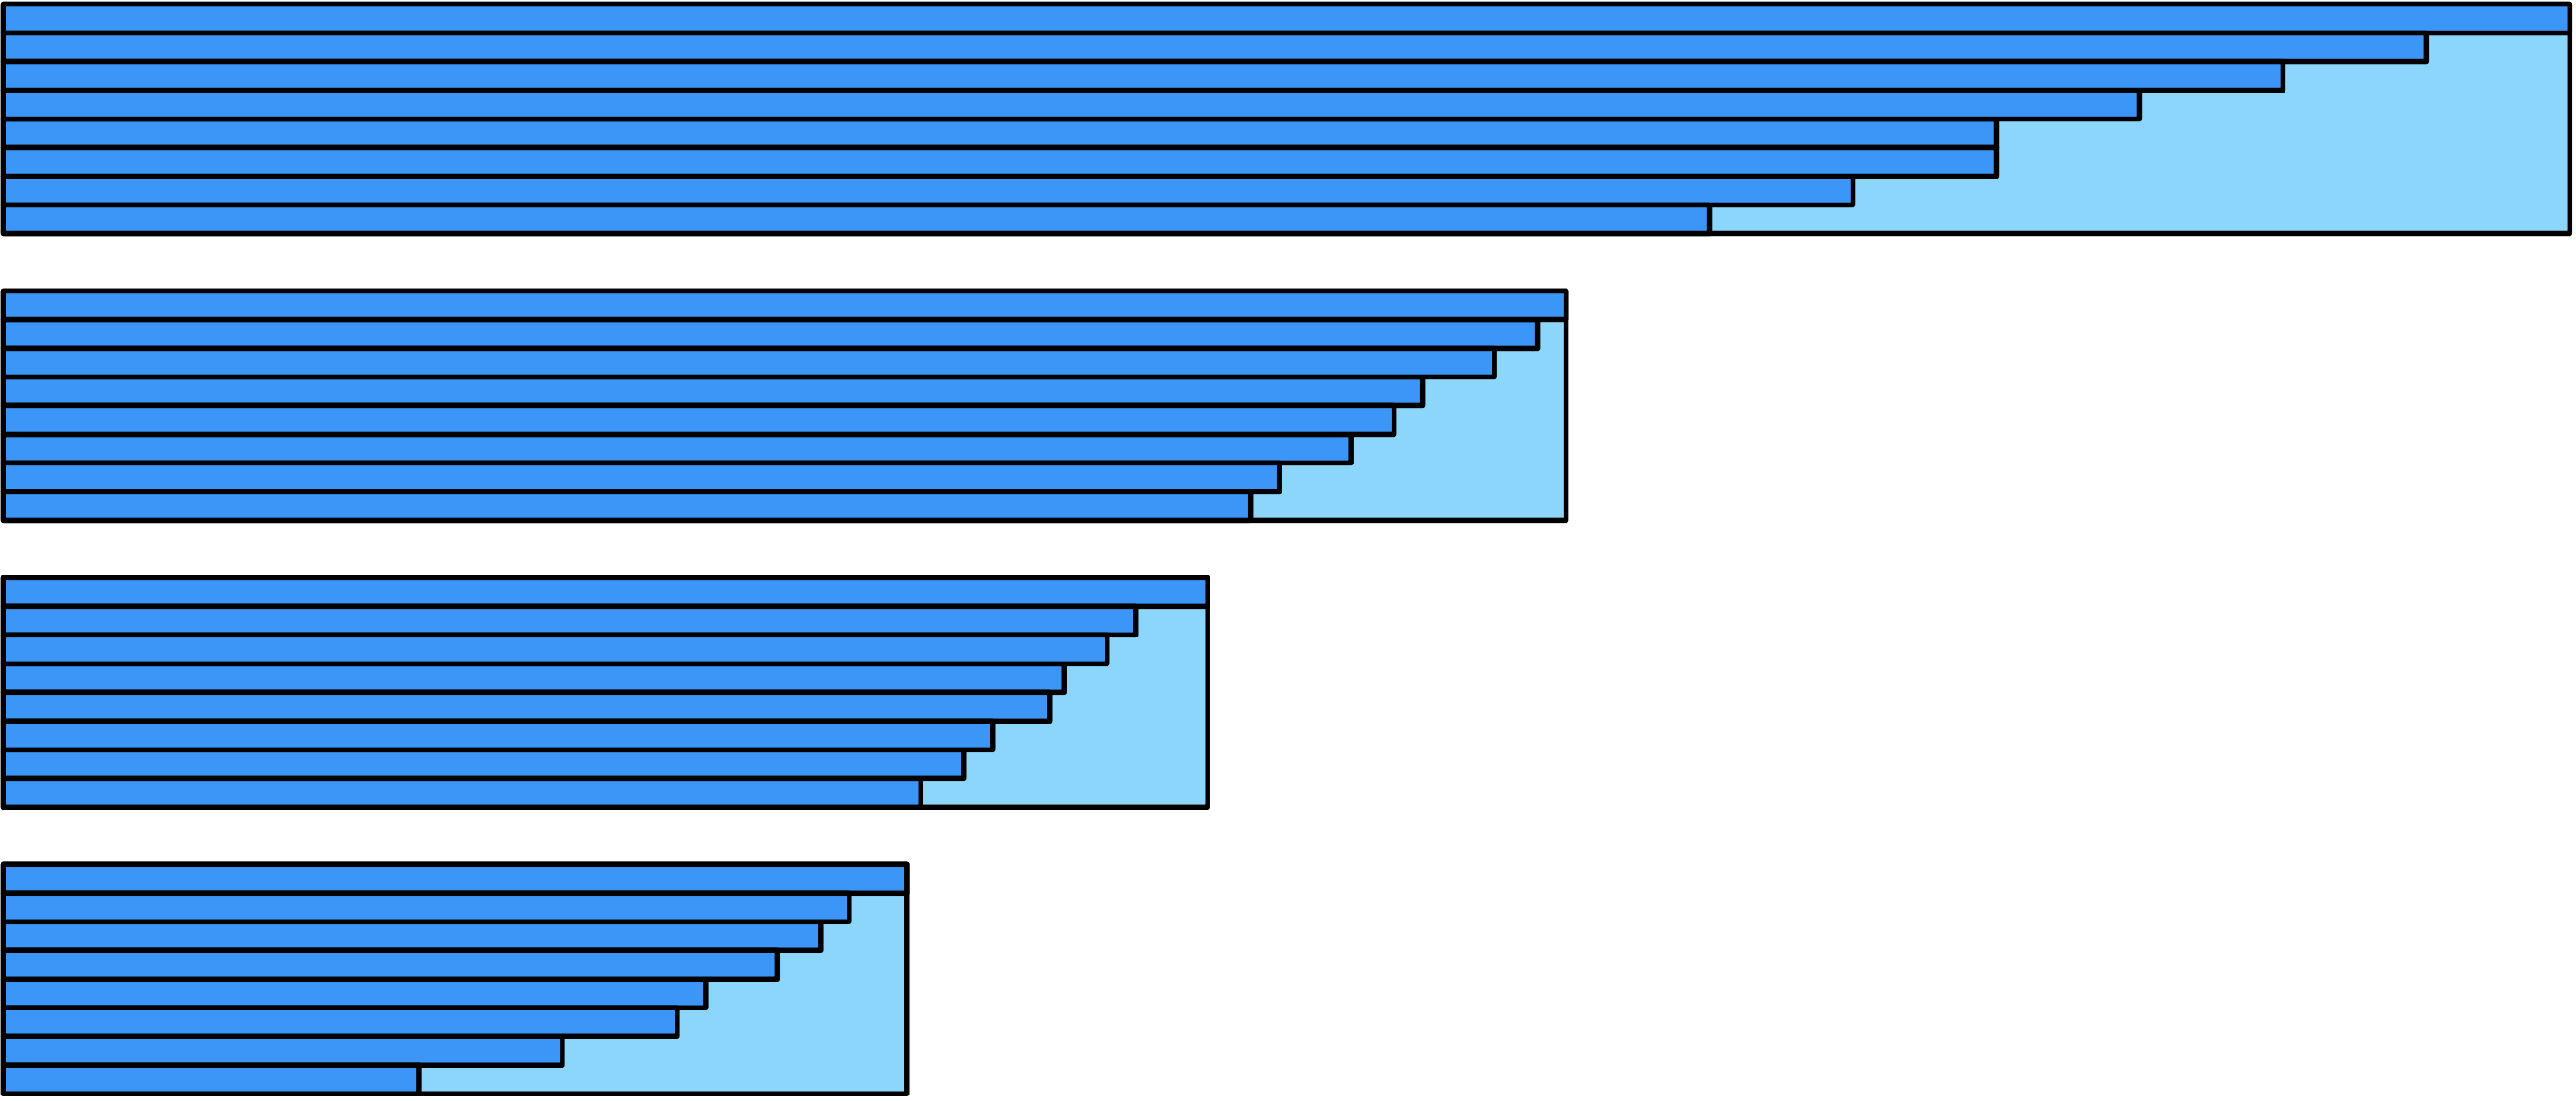
\includegraphics[width=4.5cm, valign=c]{assets/mini_batch}
\end{figure}
\begin{itemize}
  \item We can pad sentences of different lengths to increase batch size
  \item While also minimizing the use of padding
  \item Matrix Operations are faster
\end{itemize}
\end{frame}


\begin{frame}
\frametitle{Cross Entropy and Label Smoothing}
\begin{equation*}
  \text{loss}(\mathbf{x}_i, y_i) = -\underbrace{x_{y_i}}_{maximize} + \overbrace{\log \sum_j \exp x_j}^{minimize}
\end{equation*}
\begin{itemize}
  \item Softmax and Cross-Entropy loss assign all the probability mass to a single word
  \begin{itemize}
    \item LogSumExp is minimized on confidient predictions
  \end{itemize}
  \item Solution: smooth the distribution
\end{itemize}
\end{frame}


\begin{frame}
\frametitle{Cross Entropy and Label Smoothing}
\begin{itemize}
  \item Softmax
  \begin{equation*}
    p(y_i) = \frac{\exp x_{y_i}}{\sum_j \exp x_j}
  \end{equation*}
  \item Smoothed Softmax with Temperature $T$
  \begin{equation*}
    p(y_i) = \frac{\exp \left(x_{y_i} / T \right)}{\sum_j \exp \left(x_j / T \right)}
  \end{equation*}
  \item As $T \to \infty$, the distribution is smoother
\end{itemize}
\end{frame}

\begin{frame}
\frametitle{Visualizing Temperature}

\end{frame}

\begin{frame}
\frametitle{Masked Loss}

\end{frame}


%%%%%%%%%%%%%%%%%%%%%%%%%%%%%%%%%%%%%%%%%%%%%%%%%%%%%%%%%%%%%%%%%%%%%%%%%%%%%%%%
\section{Decoding: Making better Translations}

\begin{frame}
\frametitle{Beam Search}

\end{frame}

\begin{frame}
\frametitle{Monte Carlo Beam Search}

\end{frame}

\begin{frame}
\frametitle{Ensembling}

\end{frame}

\begin{frame}
\frametitle{Reranking}

\end{frame}

%%%%%%%%%%%%%%%%%%%%%%%%%%%%%%%%%%%%%%%%%%%%%%%%%%%%%%%%%%%%%%%%%%%%%%%%%%%%%%%%

\section{Tools, References, and Further Reading}


\begin{frame}
\frametitle{Refrences \& Further Reading}
  \begin{itemize}
    \item \href{https://www.cs.ubc.ca/~murphyk/MLbook/}{Machine Learning: A Probabilistic Perspective by Kevin Murphy}
  \end{itemize}
\end{frame}


% Refs, ideas, etc


\end{document}
